%!TEX root = Projeto.tex
\section{Principais conceitos}
Nesta seção são apresentados os conceitos que embasam este e outros trabalhos relacionados ao tema da segurança da informação em aplicações da web.

\subsection{Segurança da informação}
Segundo \cite{ISO2016}, segurança da informação é um processo com os objetivos de ``preservação da confidencialidade, integridade e disponibilidade da informação''. \cite{Foster1998} elabora esses objetivos, descrevendo a confidencialidade como a condição na qual a informação só pode ser acessada pelos agentes autorizados, integridade como a capacidade de proteger a informação contra modificações não autorizadas, e a disponibilidade como a capacidade de garantir acesso à informação quando necessário; \cite{Foster1998} ainda atribui mais duas características a um sistema de segurança da informação: \textit{accountability} como a possibilidade de se atribuir um agente para cada ação ocorrida dentro do sistema, e \textit{assurance} como o grau de confiabilidade na segurança do sistema em relação aos seus objetivos declarados.

Neste trabalho, qualquer definição de segurança da informação será restrita aos sistemas de informação relacionados com a navegação de usuários através da web: provedores de serviço (\textit{sites}, servidores da web), protocolos de comunicação em rede (HTTP, HTTPS, \textit{web sockets}), navegadores (\textit{browsers}) e os ambientes de execução de Javascript embutidos nos navegadores. Isto delimita a área de conhecimento relevante para este trabalho.

%\subsection{Políticas de controle de acesso}
%Segundo \cite{Goguen1982}, uma política de controle de acesso é necessária para que se estabeleçam quais fluxos de dados serão permitidos em um sistema de informação.

\subsection{Modelos de controle de acesso}
Enquanto a definição dos requisitos de segurança da informação estabelece seus objetivos, os modelos definem os sistemas derivados desses objetivos \cite{Goguen1982}. \cite{Foster1998} menciona diferentes modelos de controle de acesso, categorizados de modo amplo como modelos discricionários (DAC -- \textit{discretionary access control}) e mandatórios (MAC -- \textit{mandatory access control}). Modelos discricionários se baseiam na definição dos relacionamentos de segurança entre agentes e objetos em um sistema, como, por exemplo, a política de que um \script -- a parte \textit{agente} -- não pode iniciar conexões com domínios diferentes do seu próprio -- a parte \textit{objeto}. Modelos discricionários são os mais comumente utilizados para estabelecer mecanismos de segurança nos navegadores. O campo de atuação desses modelos é limitado aos relacionamentos de segurança estabelecidos, e portanto não podem garantir a segurança da informação quando esta ultrapassa o domínio desses relacionamentos. Isto significa, por exemplo, que dados legitimamente obtidos dentro de regras discricionárias pode ser replicado para um contexto não-seguro sem qualquer impedimento derivado do modelo de segurança.

Modelos mandatórios não atribuem explicitamente as regras de controle de acesso aos objetos e agentes de um sistema. Ao invés disso, estabelecem níveis de confidencialidade utilizados para classificar os participantes do sistema de informação, viabilizando o controle dinâmico do trânsito da informação entre os agentes. Num modelo mandatório, o nível de segurança de um dado impede que ele seja obtido ou modificado por agentes com níveis de segurança mais baixos. O controle do fluxo da informação faz dos MACs modelos mais robustos do que os DACs \cite{Foster1998}.

\subsection{Controle do fluxo de informações}
O controle do fluxo de informações (IFC -- \textit{information flow control}) é um mecanismo que atua, em tempo de execução, nos meios de propagação dos valores entre os espaços de armazenamento de um sistema computacional de modo a impedir fluxos não autorizados dos dados \cite{Denning1976}. IFC é um modelo discricionário e baseia-se em \textit{classes de segurança} ``altas'' e ``baixas'', simbolizadas pelas letras \texttt{<h>} e \texttt{<l>}, respectivamente, para indicar graus de confidencialidade das informações e dos seus espaços de armazenamento (\textit{heap}, pilha, redes, dispositivos etc). Operações entre entidades com classes de segurança diferentes, como a cópia do valor de uma variável \texttt{<h>} (confidencial) para a variável \texttt{<l>} (pública), são automaticamente impedidas de prosseguir.

IFC distingue entre fluxos de informação explícitos e implícitos. Um fluxo explícito ocorre quando uma informação classificada como ``alta'' é diretamente copiada para um contexto de classificação ``baixa'', como na listagem de código \ref{Src: jsIFCExplicitFlow}. Em um fluxo implícito, não é a informação em si que transita entre contextos de classificação diferente, mas sim alguma informação derivada dela através da qual seja possível fazer qualquer inferência sobre seu conteúdo. Um exemplo de fluxo implícito encontra-se la listagem \ref{Src: jsIFCImplicitFlow}. Um mecanismo que suporte IFC deve ser capaz de interromper vazamento de informação em ambos os tipos de fluxo.

\lstinputlisting[language=JavaScript,
inputencoding=utf8,
label={Src: jsIFCExplicitFlow},
caption={Vazamento de dados em fluxo explícito de informação}]{codigo/sample02-ifc-implicit.js}

\lstinputlisting[language=JavaScript,
inputencoding=utf8,
label={Src: jsIFCImplicitFlow},
caption={Vazamento de dados em fluxo implícito de informação}]{codigo/sample03-ifc-explicit.js}


\subsection{SOP -- Same Origin Policy}
A política de segurança SOP foi estabelecida para que os navegadores conseguissem dar suporte a páginas com conteúdo proveniente de domínios mistos com um mínimo de segurança contra o vazamento de informação entre esses domínios \cite{Hill2016}. Através desta política, os navegadores podem impedir um conjunto de ataques conhecido como \textit{cross-site resource forgery}, em que um domínio tenta instruir o navegador a fazer requisições para outro domínio em nome do usuário.

O termo \textit{origem} é intercambiável com a expressão \textit{domínio} e ambos representam, para fins desta política, componentes do endereço de URL associado com cada recurso da web -- a saber, o \textit{protocolo}, o \textit{nome do host} e a \textit{porta TCP} de onde o recurso foi transferido \cite{Barth2011}. Os exemplos a seguir representam recursos de mesma origem:

{
	\small \begin{tabular}{|l|c|l|r|}
		\hline 
		Endereço & Protocolo & Nome do \textit{host} & Porta \\ 
		\hline 
		\texttt{http://exemplo.com/} & http & exemplo.com & 80 \\ 
		\hline 
		\texttt{http://exemplo.com:80/} & http & exemplo.com & 80 \\ 
		\hline 
		\texttt{http://exemplo.com/path/file} & http & exemplo.com & 80 \\ 
		\hline 
	\end{tabular}
}


Os endereços a seguir representam recursos de origens diferentes:

{\small
	\begin{tabular}{|l|c|l|r|}
		\hline 
		Endereço & Protocolo & Nome do \textit{host} & Porta \\ 
		\hline 
		\texttt{http://exemplo.com/} & http & exemplo.com & 80 \\ 
		\hline 
		\texttt{http://exemplo.com:8080/} & http & exemplo.com & 8080 \\ 
		\hline 
		\texttt{http://www.exemplo.com/} & http & www.exemplo.com & 80 \\ 
		\hline 
		\texttt{https://exemplo.com:80/} & https & exemplo.com & 80 \\ 
		\hline
		\texttt{https://exemplo.com/} & https & exemplo.com & 443 \\ 
		\hline
		\texttt{http://exemplo.org/} & http & exemplo.org & 80 \\ 
		\hline
	\end{tabular}
}

Segundo a SOP, as atividades derivadas da inclusão de recursos de origens mistas são categorizadas em três ações \cite{Ruderman2017}:

\begin{alineas}
	\item \textbf{Escrita:} atividades deste tipo instruem o navegador para que ocorra alguma forma de navegação entre páginas, o que inclui a interação com \textit{links}, redirecionamento e submissão de formulários. Em geral SOP não restringe este tipo de ação;
	\item \textbf{Incorporação:} SOP permite que recursos incorporados à página tenham origens mistas. Isto significa que é possível a inclusão de imagens, vídeos, \scripts e do elemento \texttt{<iframe>}, entre outros, provenientes de origens mistas e dentro de uma mesma página.
	\item \textbf{Leitura:} atividades de leitura permitiriam que o conteúdo dos recursos carregados pudesse ser consultado entre origens. SOP permite que um subconjunto de funcionalidades de leitura possam ocorrer entre domínios diferentes.
\end{alineas}

Um aspecto importante da SOP é o tratamento dado a \scripts incorporados. Quando uma página inclui um \script proveniente de outras origens, por exemplo pelo uso de uma CDNs (\textit{content distribution networks}), esses \scripts são executados em contexto da origem do documento em que eles foram incorporados. Isto permite, por exemplo, que \textit{frameworks} populares como jQuery e Angular.js possam ser disponibilizados em CDNs sem perder funcionalidades importantes, como a capacidade de iniciar chamadas assíncronas pela técnica AJAX. Esta concessão da SOP, porém, abre a possibilidade de que esses scripts, se adulterados, executem atividades maliciosas sem impedimentos.

\subsection{CSP -- Content Security Policy}
CSP foi criada como um complemento à SOP, elevando a capacidade do navegador de servir como plataforma razoavelmente segura para composição de aplicações \textit{mashup} ao estabelecer um protocolo para o compartilhamento de dados entre os componentes da página que residam em domínios diferentes. CSP define um conjunto de diretivas (codificadas como cabeçalhos HTTP) para a definição de \textit{whitelists} -- o conjunto de origens confiáveis em um dado momento -- pelas quais navegador e provedores de conteúdo estabelecem o controle de acesso e o uso permitido de recursos embutidos como \scripts, folhas de estilos, imagens e vídeos, entre outros. Através desse protocolo, ataques de XSS que podem ser neutralizados desde que todos os componentes na página sejam aderentes à mesma política de CSP.

\subsection{CORS -- Cross-Origin Resource Sharing}
Assim como a CSP, o mecanismo CORS \cite{W3C:CORS} complementa a SOP estabelecendo um conjunto de diretivas (cabeçalhos HTTP) para a negociação de acesso via Ajax/XHR a recursos hospedados em domínios diferentes. CORS determina que exista um vínculo de confiança entre navegadores e provedores de conteúdo, dificultando vazamento de informação ao mesmo tempo em que flexibiliza as funcionalidades das APIs. O uso de CORS permite que os autores de componentes e desenvolvedores de aplicações \textit{mashup} determinem o grau de exposição que cada conteúdo pode ter em relação aos outros conteúdos incorporados.

CSP e CORS são recomendações do comitê W3C \cite{W3C:CSP} \cite{W3C:CORS}, sendo incorporados por todos os navegadores relevantes desde 2016 \cite{CanIUse:CSP} \cite{CanIUse:CORS}.

\subsection{Vulnerabilidades}
Violações de privacidade são possíveis nos navegadores por causa da natureza dinâmica da linguagem Javascript e de sua ausência de restrições de segurança em tempo de execução \cite{Jang2010}. Seus usuários estão expostos a ataques sutis com objetivos diversos como roubar \textit{cookies} e \textit{tokens} de autorização, redirecionar o navegador para sites falsos (\textit{phishing}), observar o histórico de navegação e rastrear o comportamento do usuário através dos movimentos do ponteiro do mouse e eventos de teclado. Para que \scripts mal-intencionados sejam incorporados a páginas benignas, \textit{hackers} fazem uso de vulnerabilidades como \textit{cross-site scripting (XSS)} \cite{OWASP:XSS} e comprometimento de extensões \cite{Heule2015_Most_Dangerous_Code} do navegador.


\subsubsection{Compartilhamento do ambiente de execução}
Código \textit{inline} ou \scripts baixados pelas páginas da web são executados com os mesmos privilégios e mesmo nível de acesso à estrutura de documento do navegador, o chamado DOM (\textit{document object model}) \cite[p. 2-3]{DeRyck2012}, não importando o domínio de origem dos \scripts. Uma demonstração do problema pode ser exemplificada na figura \ref{Fig: diagrama01} e listagem de código \ref{Src: webPageMultiOrigin}. Nesse exemplo, um \script tido como benigno é incorporado a uma página web a partir de um domínio de CDN (\textit{content delivery network}), diferente daquele da aplicação que efetivamente publica a página. O servidor da página, pelo protocolo CORS, sinaliza ao navegador que o domínio da CDN é confiável. O \script externo pode, então, iniciar requisições ao seu domínio de origem -- uma consequência desejada pelos autores da página, pois o \script depende desse acesso para efetuar suas funções.

\begin{figure}
	\centering
	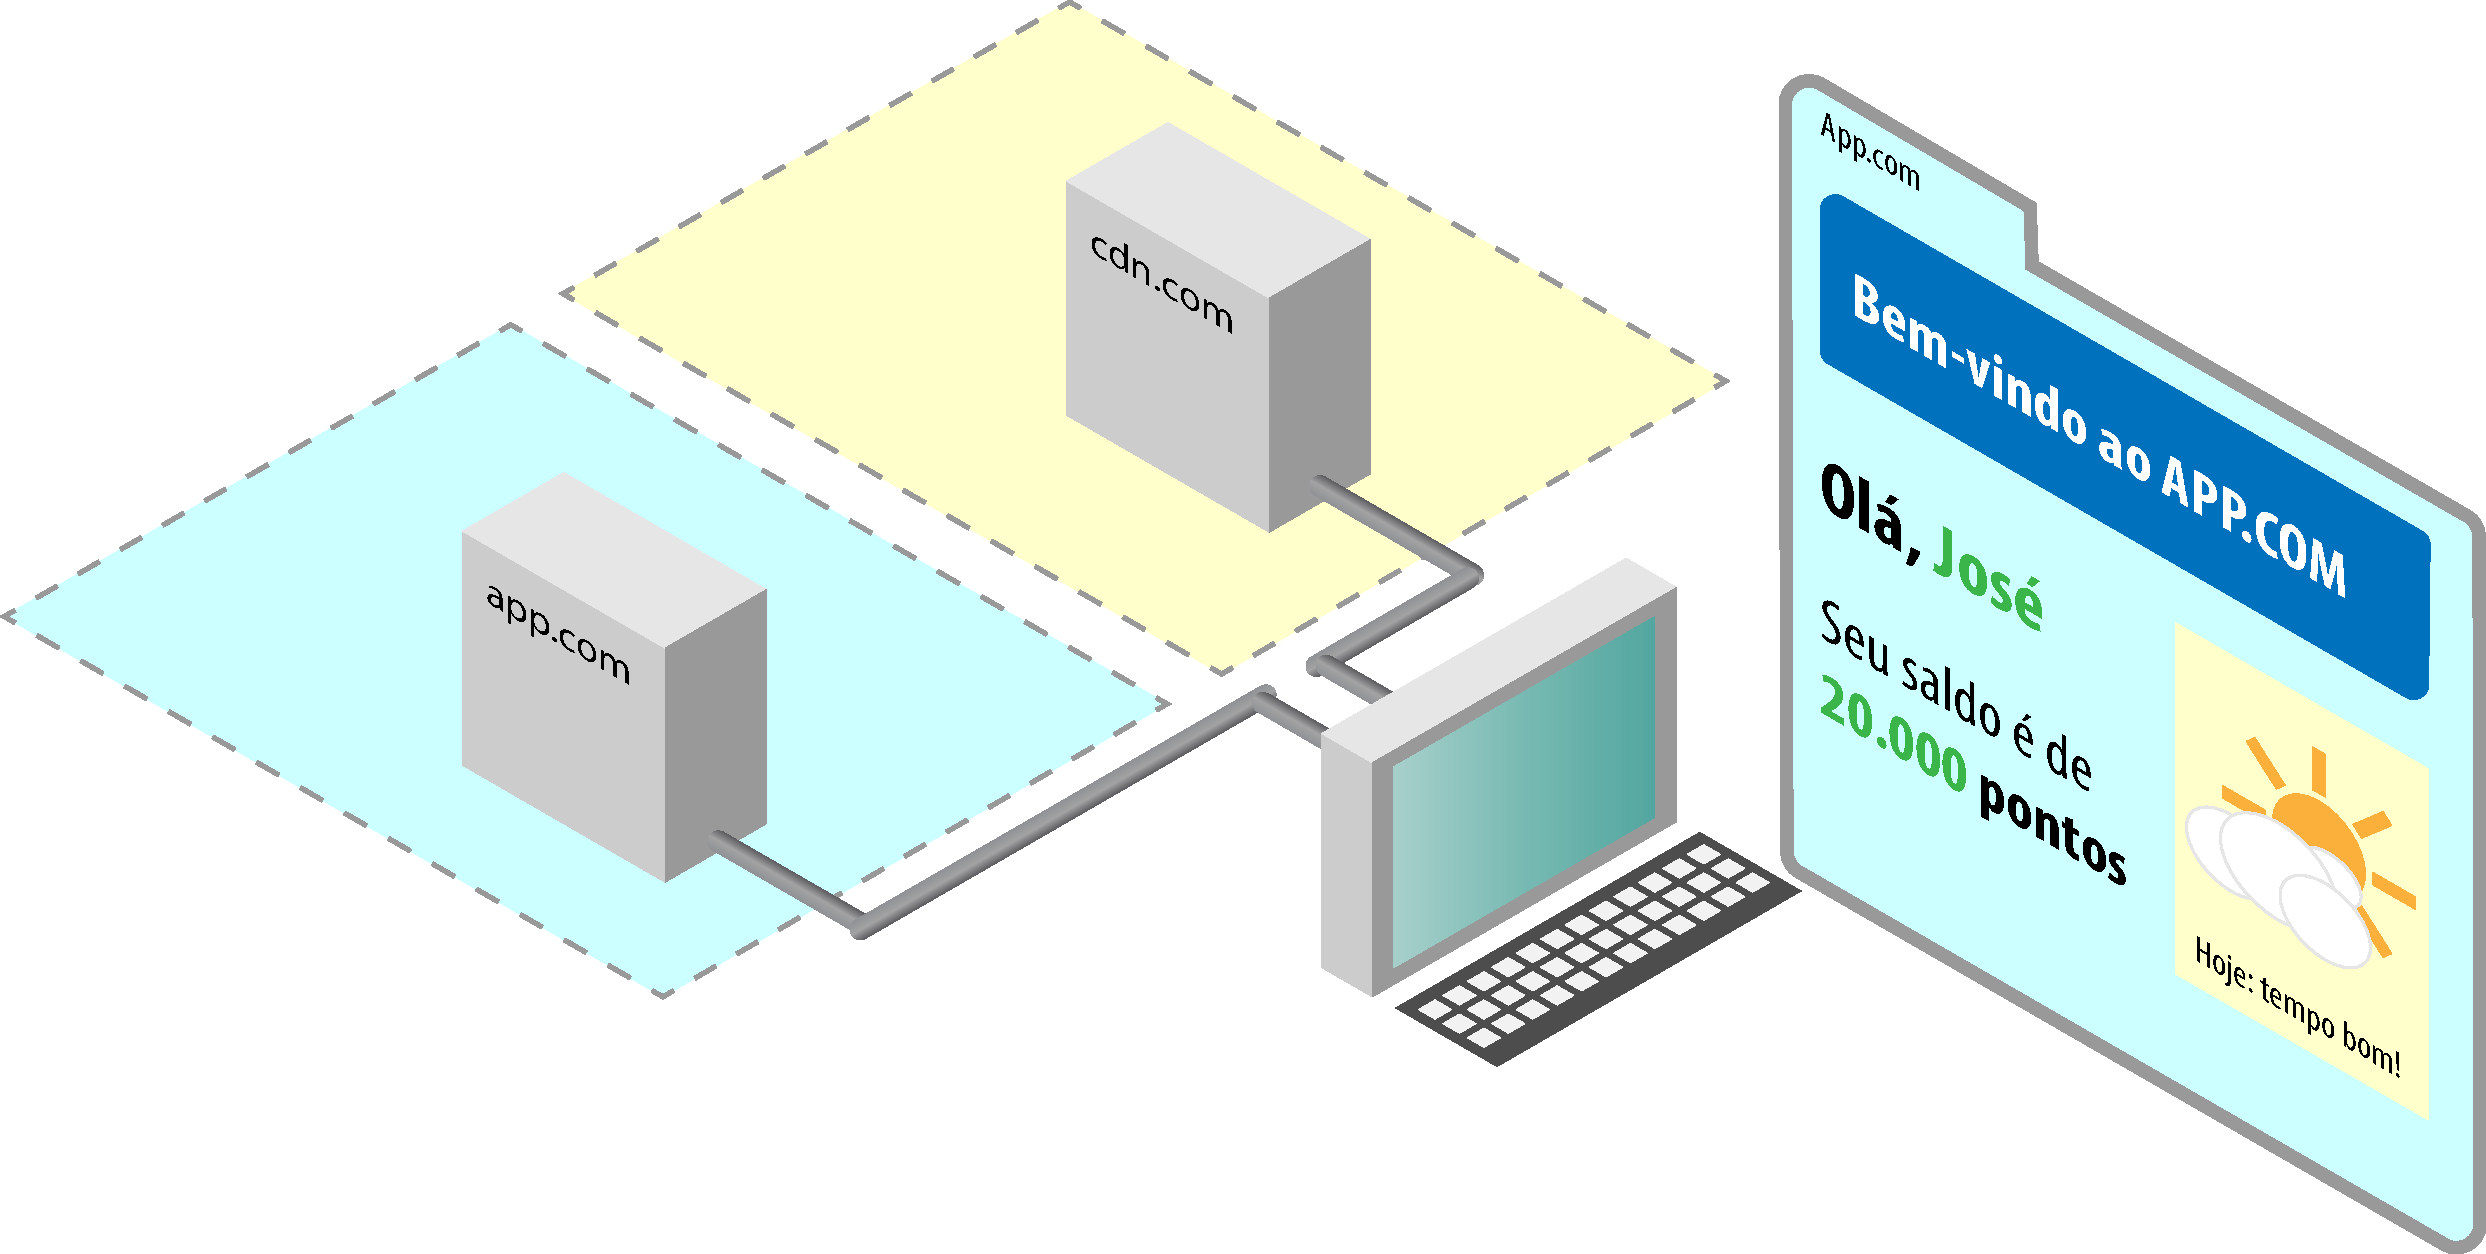
\includegraphics[width=10cm]{diagramas/diagrama01.pdf}
	\caption{Aplicação web composta por conteúdo proveniente de duas origens.}
	\label{Fig: diagrama01}
	
	\lstinputlisting[language=html,
	inputencoding=utf8,
	label={Src: webPageMultiOrigin},
	caption={[Página HTML incorporando \script de outra origem]Incorporação de \script de outra origem (linha \ref{lstCdnScript})}]{codigo/sample01-leaking-script.html}
\end{figure}

Em momento posterior, o \script servido pelos servidores da CDN é substituído por código malicioso que, além de efetuar as funções do \script benigno, captura o conteúdo da página armazenado no DOM \ref{Fig: diagrama02}. O \script pode buscar informações específicas e potencialmente sensíveis como identificação do usuário, senhas e endereços. Por causa da autorização concedida pelo protocolo CORS, o código mal intencionado tem a chance de transmitir o conteúdo capturado para um serviço anômalo.

\begin{figure}
	\centering
	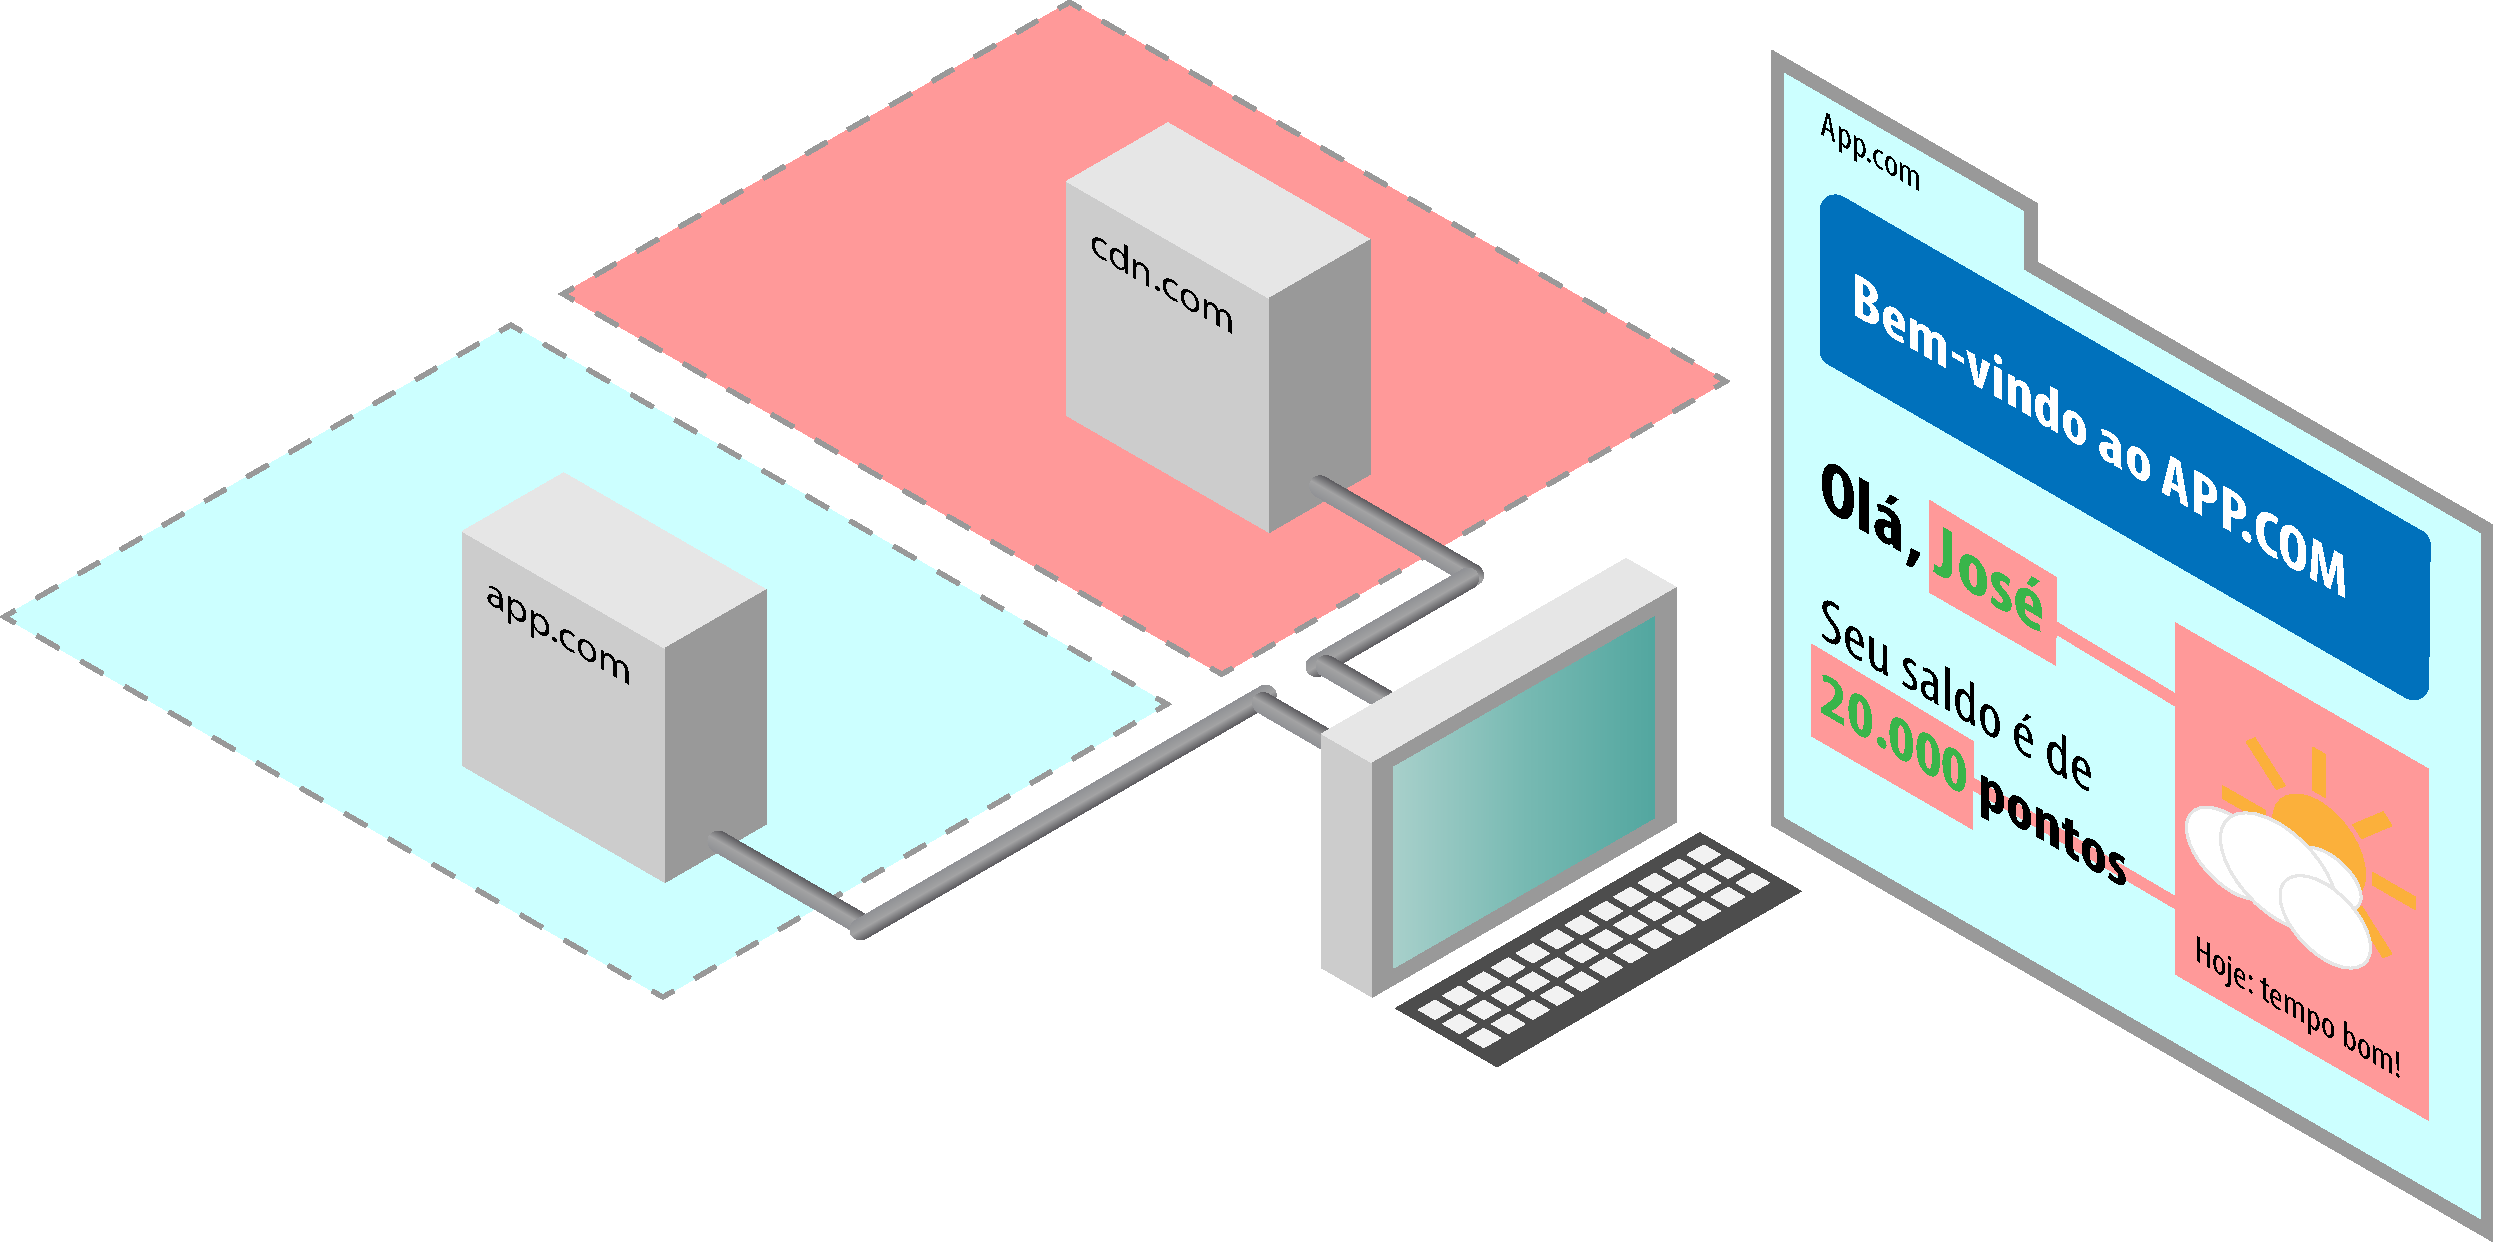
\includegraphics[width=10cm]{diagramas/diagrama02.pdf}
	\caption{Domínio de CDN comprometido, capturando informações do usuário.}
	\label{Fig: diagrama02}
\end{figure}

Acessar, capturar e modificar informações contidas no DOM também são efeitos de extensões do navegador. Mas, diferentemente dos \scripts incorporados em páginas, extensões são executadas em modo privilegiado e podem afetar todas as páginas carregadas pelo navegador, não sendo confinadas a domínios específicos. Extensões como as do Google Chrome são publicadas exclusivamente em site específico e protegido, mas não é impossível que o código fonte de extensões seja descaracterizado e publicado pela ação de \textit{hackers} \cite{Spring2017}, afetando a todos os usuários que atualizarem a extensão -- um processo automático por padrão \cite{Google2017}.


\subsubsection{Cross-Site Scripting (XSS)}
Em Javascript, todos os recursos de código carregados dentro de uma mesma página possuem os mesmos privilégios de execução. Ataques do tipo \textit{cross-site scripting} tiram proveito dessa característica para injetar código malicioso em contextos onde seja possível observar e retransmitir informação sigilosa como \textit{cookies} do usuário, endereço do navegador, conteúdo de formulários, ou qualquer outra informação mantida pelo DOM.

O emprego de medidas para prevenção de ataques XSS \cite{OWASP:XSS-CheatSheet} não elimina riscos inerentes à tecnologia do navegador. Uma vez que componentes incorporados, como anúncios e \textit{players} de mídia, conseguem carregar \scripts tidos como confiáveis dinamicamente, um único trecho de código comprometido pode colocar informações em risco sem qualquer interferência dos dispositivos de segurança.

%\subsubsection{Sobrescrita do DOM} DOM CLOBBERING

\subsubsection{Comprometimento de extensões}
Os mecanismos de extensibilidade oferecidos pelos navegadores melhoram a funcionalidade da web para os usuários, e o código de que são feitos é executado com privilégios mais elevados do que o dos \scripts incorporados pelos \textit{sites}. Por isso, os usuários precisam confirmar ao navegador que aceitam que uma extensão seja instalada, sendo informados a respeito dos privilégios que a extensão pretende utilizar. O fato de que esse processo precisa se repetir a cada vez que uma extensão necessita de um conjunto de privilégios diferente faz com que os desenvolvedores optem por solicitar, de antemão, uma gama de privilégios maior que a estritamente necessária \cite{Heule2015_Most_Dangerous_Code}.

Uma extensão que tiver sido comprometida (por exemplo, ao usar \scripts de terceiros que, por sua vez, tenham sido redirecionados ou adulterados) terá assim poder para ler e transmitir todo o conteúdo carregado e exibido pelo navegador, com o potencial de causar os mesmos efeitos observados em um ataque XSS, mas em escopo e poder aumentados, já que poderiam afetar todas as páginas abertas e todas as APIs publicadas pelo navegador.
